\chapter{Disposiif expérimental}
\mylocaltoc


\section{Introduction du chapitre}\label{chap:IntroProtocExp}
Après avoir brièvement rappelé les bases de fonctionnement des machines thermoacoustiques, il est temps de décrire le réfrigérateur support de cette thèse. Le choix de la géométrie, les paramètres hydrauliques du régénérateur utilisé, et enfin la chaîne d'excitation et d'acquisition sont présentés dans la section~\ref{chap:PresentationTacot} - \nameref{chap:PresentationTacot}. La deuxième partie présente les conditions expérimentales choisies ainsi que le protocole suivi pour chaque mesure dans la section~\ref{chap:ProtocolExpe} - \nameref{chap:ProtocolExpe}.
%Les simulations théoriques réalisées sont ensuite expliquées en troisième partie, dans la section~\ref{chap:SimusRealisees} (\nameref{chap:SimusRealisees}).

%Ces parties visent à créer une vue d'ensemble de ce qui est fait durant cette thèse et le présenter de manière globale pour pouvoir s'y référer dans les différents chapitres suivants.

\section{Présentation du dispositif expérimental actuel}\label{chap:PresentationTacot}

\subsection{Résultats déjà obtenus}\label{chap:PresTacot_ResultatsATE}
\echaf{Quelques résultats. À mettre dans l'intro I ?} Au démarrage de cette thèse, le réfrigérateur existe déjà et sa caractérisation est publiée \cite{ramadan_design_2021}, et fait également l'objet d'études expérimentales~\cite{ramadan_experimental_2018, ramadan_experimental_2021} et  numériques~\cite{hireche_numerical_2019, hireche_experimental_2020,}. Dans cet article, il est montré que la fréquence de fonctionnement offrant les meilleures performances est $f=\qty{47}{\hertz}$, soit la première fréquence de résonance du système, et avec un déphasage inter-sources $\phi_{2-1}=\qty{-60}{\degree}$. À ce point de fonctionnement et à une puissance d'alimentation des sources $\dot W_e=\qty{193}{\watt}$ soit un \textit{drive ratio} $DR=\qty{3.6}{\percent}$, une quantité de chaleur de $\dot Q_f=\qty{290}{\watt}$ est extraite à la source froide dont la température est $T_a=\qty{15}{\degreeCelsius}$. Le coefficient de performance est $\COP=\num{1.5}$, soit \qty{15}{\percent} du coefficient de performance de Carnot. \echaf{ajouter figures des écarts mesures-modèle DeltaEC}

\subsection{Géométrie du réfrigérateur \textsc{Tacot}}
\subsubsection{Cavité thermoacoustique}
La pompe à chaleur a été dimensionnée et fabriquée dans le cadre du projet ANR \textsc{Tacot} (ThermoAcoustic Cooler for Onroad Transportation), qui porte sur l'application d'une pompe à chaleur thermoacoustique pour la climatisation automobile \cite{ANR_thermo-acoustic_2019}. Ce projet apporte beaucoup de contraintes, dont l'une des principales est la compacité. Contrairement aux autres systèmes thermoacoustiques existant et bien plus volumineux (tels que le liquéfacteur de gaz naturel développé par Swift et Wollan au Los Alamos National Laboratory \cite{swift_thermoacoustics_2002, wollan_development_2002}, ou le réfrigérateur cryogénique thermoacoustique spatial (STAR) \cite{adeff_measurement_1991, garrett_thermoacoustic_1993}), les dimensions doivent être réduites tout en conservant un pompage de chaleur efficace. Pour cela, une géométrie coaxiale pour la cavité thermoacoustique est préférée à celle toroïdale usuellement utilisée en suivant les travaux de Poignand \textit{et al.} \cite{poignand_thermoacoustic_2011, poignand_analysis_2013}. L'ajout d'une source acoustique secondaire dans la cavité thermoacoustique permet également de gagner en compacité, en remplaçant un résonateur plus long par la masse de son équipage mobile et la souplesse de sa suspension, tel que réalisé dans les travaux de Poese \textit{et al.} \cite{poese_thermoacoustic_2004}. En plus de permettre une diminution du volume de la machine, utiliser une source secondaire offre plus de flexibilité qu'un résonateur sur la relation entre pression acoustique et vitesse particulaire, et facilite en particulier le ciblage du déphasage optimal entre pression et vitesse acoustiques au sein du noyau thermoacoustique. Un schéma général présente la géométrie de la pompe à chaleur sur la figure~\ref{fig:SchemaGeneralTACOT}, adapté de Ramadan \textit{et al.} \cite{ramadan_design_2021}. 

\begin{figure}[!ht]
    \centering
    \external{fig_SchemaGeneralTACOT}
%    \externalremake
    \begin{tikzpicture}[scale=.5]
	\node[anchor=south west, inner sep=0] (image) at (0,0) {\includegraphics[angle=0,origin=c,width=.6\textwidth]{../fig/fig_TACOTSchematics/TACOT.png}};
	
	\node[anchor=east, inner sep=0] (imagecropped) at (image.west) {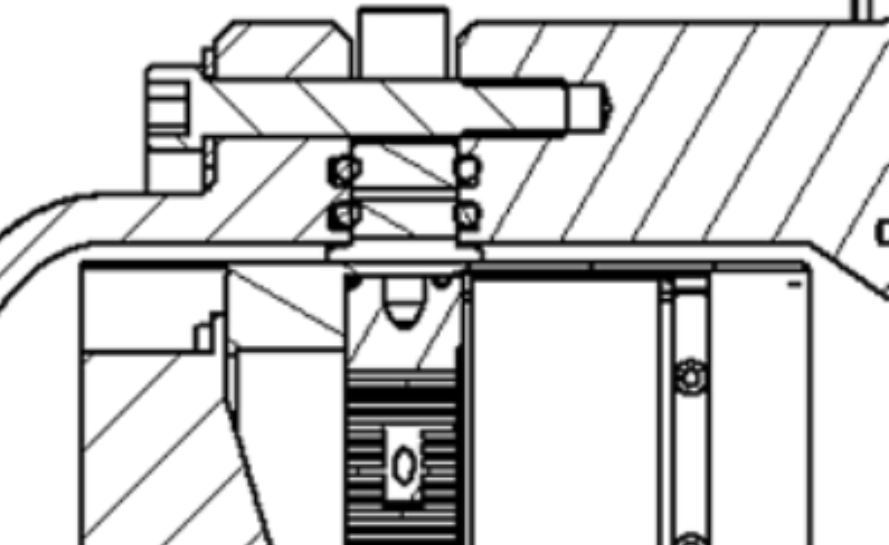
\includegraphics[angle=0,origin=c,width=.35\textwidth]{../fig/fig_TACOTSchematics/TACOT_Cropped.png}};

\draw[black, very thick, dashed, rounded corners] (imagecropped.north west) rectangle (imagecropped.south east);
%\draw[black, very thick, dashed, rounded corners] ($(AHX)+(-1.5cm,3cm)$) rectangle ($(CHX)+(.75cm,-.5cm)$);
	
	\begin{scope}[x={(image.south east)},y={(image.north west)}]
	
%		\filldraw (0,0) circle (2pt); 
%		\filldraw[green] (1,0) circle (1pt);
%		\filldraw[red] (1,1) circle (1pt);		
%		\filldraw[blue] (0,1) circle (1pt);
%		\draw[help lines,xstep=.1,ystep=.1] (0,0) grid (1,1);
%		\fill[orange, rounded corners, opacity=1,draw=orange] (.46,.65) -- ++(132:.09) -- ++(0,-.44) -- ++(48:.09) -- cycle;
		\draw[MatlabYellow,rounded corners,very thick,preaction={fill=MatlabYellow!20,opacity=.5}] (.46,.65) -- ++(132:.09) -- ++(-.03,0) -- ++(0,-.44) --++(.03,0) -- ++(48:.09) -- cycle; %node[left,pos=.5,label={[rotate=90]center:Cavité}]{};
		\draw[MatlabYellow] (.415,0.5) node [label={[rotate=90]center:\textbf{Cône}}]{};
		
%		\draw[blue] (.5,.5) node [anchor=center, preaction={fill=black!20,opacity=.7}] {RIX};
%		\draw[red] (.33,.5) node [anchor=center, preaction={fill=black!20,opacity=.7}] {TA core};	
	
		\draw[MatlabPurple,rounded corners,very thick,preaction={fill=MatlabPurple!20,opacity=.5}] (.365,.7) rectangle (.245,.3) node[pos=.5,label={[rotate=90]center:\textbf{Noyau}}]{};
		
		\node (AHX) at (.27,.65) {};
		\node (Reg) at (.32,.65) {};
		\node (CHX) at (.36,.65) {};
		\node (RIX) at (.77,.4) {};

		\node (HP) at (.19,.4) {};
		
		\draw[<-,very thick,MatlabOrange] (AHX.center) to[out=90,in=0] ($(AHX)+(-.2,.41)$) node[left]{\begin{tabular}{r} Echangeur de chaleur ambiant \\ (HXA) \end{tabular}};		
		\draw[<-,very thick] (Reg.center) to ($(Reg)+(0,.4)$) node[above]{Régénérateur};
		\draw[<-,very thick,MatlabBlue] (CHX.center) to[out=90,in=180] ($(CHX)+(.2,.41)$) node[right]{\begin{tabular}{l} Echangeur de chaleur froid \\ (HXF) \end{tabular}};
		
		\draw[->,very thick,green!50!black] ($(RIX)+(0,-.4)$) -- (RIX.center) node[pos=0,anchor=north]{\begin{tabular}{c}Source acoustique principale \\ (SA1) \end{tabular}};
		\draw[->,very thick,green!50!black] ($(HP)+(0,-.4)$) -- (HP.center) node (SA2) [pos=0,anchor=north]{\begin{tabular}{c}Source acoustique secondaire \\ (SA2) \end{tabular}};
		
%		\draw [white] (.455,.5) node{+};
%		\draw [white] (.41,.65) node{+};
%		\draw [white] (.41,.5) node{+};
%		\draw [white] (.41,.35) node{+};

		\draw[black, very thick, dashed, rounded corners] ($(AHX)+(-.14,.2)$) node(a){} rectangle ($(CHX)+(.07,-.1)$);
		
		\draw[black, very thick, dashed] (a) -- (imagecropped.north east);
		\draw[black, very thick, dashed] ($(a)+(0,-.3)$) -- (imagecropped.south east);
		

	\end{scope}
	
	\draw(imagecropped.south) node[below]{\small \textbf{(a)}};		
	\draw(SA2.south -| image.south) node{\small \textbf{(b)}};
	
\end{tikzpicture}
    \caption{Schéma général du réfrigérateur \textsc{Tacot}.}
    \label{fig:SchemaGeneralTACOT}
\end{figure}

\subsubsection{Noyau thermoacoustique}
Tout comme la machine qui le contient, le noyau adopte une géométrie cylindrique et est composé d'un régénérateur représenté sur la figure~\ref{fig:TacotPhotos_Regen} encadré par deux échangeurs de chaleur. Le premier est l'échangeur ambiant et a pour rôle d'extraire la chaleur qui s'accumule de ce côté du noyau, afin d'éviter l'échauffement global de la machine. Le second est l'échangeur froid, et sa fonction et de simuler une charge thermique à refroidir. Ces échangeurs sont représentés respectivement sur les figures~\ref{fig:TacotPhotos_AHX} et \ref{fig:TacotPhotos_CHX}. Ces trois éléments sont ensuite montés dans une enceinte cylindrique qui se fixe sur le bâti de la machine pour maintenir l'espace nécessaire à la boucle de rétroaction.

\begin{figure}[!ht]
    \centering
	\begin{subfigure}{.32\textwidth}
		\centering
\includegraphics[width=\textwidth]{../fig/fig_TacotPhotos/AHX_dansCarter.JPG}
		\caption{}
		\label{fig:TacotPhotos_AHX}
	\end{subfigure}		
	\begin{subfigure}{.32\textwidth}
		\centering
\includegraphics[width=\textwidth]{../fig/fig_TacotPhotos/Regenerateur.JPG}
		\caption{}
		\label{fig:TacotPhotos_Regen}
	\end{subfigure}	
	\begin{subfigure}{.32\textwidth}
		\centering
\includegraphics[width=\textwidth]{../fig/fig_TacotPhotos/CHX_dansCarter.JPG}
		\caption{}
		\label{fig:TacotPhotos_CHX}
	\end{subfigure}	    
    \caption{Composition du noyau thermoacoustique. \subref{fig:TacotPhotos_AHX} \'Echangeur ambiant, \subref{fig:TacotPhotos_Regen} régénérateur, et \subref{fig:TacotPhotos_CHX} échangeur froid.}
    \label{fig:TacotPhotos}
\end{figure}


Les axes $\mathbf e_x$ et $\mathbf e_r$ sont alors respectivement associés aux directions axiale et radiale du noyau, \echaf{J'arrive pas à relire} avec pour sens positive choisie dans le sens de l'échangeur froid vers l'échangeur ambiant pour le premier, et du centre du noyau vers l'extérieur pour le second.\medskip

Le régénérateur est composé de \echaf{combien} disques de tissus métalliques (Gantois, modèle : 102045) empilés dans une enceinte cylindrique de diamètre intérieur $D_{\sf reg}=\qty{148}{\mm}$ et de longueur $L_{\sf reg}=\qty{39}{\mm}$ pour atteindre la porosité $\Phi~=~\qty{68}{\percent}$. Un noyau de cette porosité doit être comparé avec le noyau support des expériences dont les résultats sont publiés par Ramadan \textit{et al.} et dont la porosité vaut \qty{75}{\percent} \cite{ramadan_design_2021}. La quantité de tissus à utiliser pour atteindre la porosité souhaitée s'obtient en utilisant la relation

\begin{align}
	\Phi &= \frac{V_{\sf gaz}}{V_{\sf tot}}, \label{eq:Porosite_Volume}%\\
%	&= \frac{V_{\sf tot}-V_{\sf metal}}{V_{\sf tot}} \nonumber\\
%	&= 1 - \frac{m_{\sf metal}}{m_{\sf tot}} \label{eq:Porosite_Masse}
\end{align}
où $V_{\sf gaz}$ représente le volume occupé par le gaz dans le régénérateur, et $V_{\sf tot}$ le volume total du régénérateur. Le milieu ainsi constitué est poreux et tortueux car l'orientation des disques de tissus est aléatoire, et le rayon hydraulique est défini par \cite{swift_thermoacoustics_2017} %\echaf{ajouter source pour justifier que les matériaux type "mousse" se comporte comme du cylindrique : UPDATE dans Swift TA unifying... chapitre 7 (tortuous porous media)}

\begin{equation}
	r_h = d_w\frac{\Phi}{4(1-\Phi)},
	\label{eq:DefRayonHydrauGantois}
\end{equation}
avec $d_w$ le diamètre du fil. Ce milieu poreux dispose d'une certaine capacité à laisser passer un écoulement. C'est la perméabilité notée $K_p$, qui est définie par 

\begin{equation}
	K_p = \echaf{\frac{4 r_h^2 \Phi}{8}},
	\label{eq:DefPermeabilite_LISN}
\end{equation}
\echaf{d'après le excel du LISN} \cite{hireche_experimental_2020}, ou

\begin{equation}
	K_p = \echaf{v_{\sf ref}\frac{\nu \Delta x}{\Delta P}},
	\label{eq:DefPermeabilite_Wikipedia}
\end{equation}
\echaf{d'après la formulation générale} \cite{nield_convection_2013}.

Les dimensions et paramètres du régénérateur sont résumés dans le tableau \ref{tab:ParamHydrauTAC}.

\begin{table}[!ht]
    \caption{Paramètres hydrauliques du régénérateur à la fréquence de fonctionnement, \linebreak $f=\qty{47}{\Hz}$}
    \label{tab:ParamHydrauTAC}
    \centering
    \begin{tabular}{l@{\hspace{1cm}}l}
    	\hline
    	\textbf{Paramètre [unité]} & \textbf{Valeur} \\\hline\hline
    	Diamètre du noyau $D_{\sf reg}$ [\unit{\meter}] & \num{148e-3} \\
    	Longueur du régénérateur $L_{\sf reg}$ [\unit{\meter}] & \num{39e-3} \\
    	Diamètre du fil $d_w$ [\unit{\meter}] & \num{53e-6} \\
        Rayon hydraulique $r_h$ [\unit{\meter}] & \num{2.81e-5} \\
        Porosité du noyau $\Phi$ [\unit{\percent}] & \num{68}\\
        Couche limite thermique $\delta_\kappa$ [\unit{\meter}] & \num{1.4452e-4} \\
        Couche limite visqueuse $\delta_\nu$ [\unit{\meter}] & \num{9.1120e-5} \\
        \echaf{Perméabilité} [\unit{\meter\squared}] & \num{2.68e-10} \\
        \hline
    \end{tabular}
\end{table}

Cette machine nécessite entre autres choses le respect de la condition $\delta_{\kappa,\nu} \gg r_h$, de sorte à avoir un excellent contact thermique entre le fluide et le solide poreux. Pour le fluide considéré, les épaisseurs de couches limites sont tracées en fonction de la fréquence et comparé au rayon hydraulique sur la figure~\ref{fig:dKdV}.

\begin{figure}[!ht]
    \centering
    \external{fig_dKdV}
%    \externalremake
    \begin{tikzpicture}
    \def\width{.9*\textwidth};
    \def\height{.45*\width};
    \def\spx{.25cm};
    \def\spy{1.25cm};
    \def\legx{.5cm};
    \def\legy{\legx};
    \def\prop{.45};
    \def\xcursor{47};
    \def\ycursorV{9.112e-5};
    \def\ycursorK{1.4452e-4};
    \def\rh{2.81e-5};
    
    \begin{axis}[name=dKdV,width={\width},height={\height},
    grid=both, minor tick num=10, 
    grid style={line width=.1pt, draw=gray!10},
    major grid style={line width=.2pt,draw=gray!50},
    xlabel={Fréquence $f$ [\unit{\Hz}]},
    ylabel={\'Epaisseurs de couches limites $\delta_{\kappa,\nu}$ [\unit{\m}]},
    xmin=0,xmax=75,ymin=0,ymax=.5/1000,
    xtick={0,25,50,75,100},
    extra x ticks={47},
    extra x tick style={
        grid=major,
        xticklabel={\num{47}},
        xticklabel style={yshift=0, anchor=north}
        },
    extra y ticks={\rh},
    extra y tick style={
        grid=major,
        yticklabel={$r_h$},
        yticklabel style={yshift=1mm, anchor=east}
        },
    ytick={0,1e-4,...,10e-4},
%    ytick={0,2.81/100000,9.1120/100000,1.4452/10000,
%    	2.5/10000,5/10000,1/1000},
    scaled y ticks = false,
    domain=0:100,
    legend cell align={left},
    legend style = {at={($(1,1)+(-2mm,-2mm)$)},anchor = north east,rounded corners}
    ]
        \addplot[solid,ultra thick,draw=Plasma1] file {../fig/fig_dKdV/data/data_dK.txt};
        \addplot[solid,ultra thick,draw=Plasma64] file {../fig/fig_dKdV/data/data_dV.txt};
        \filldraw[Plasma1] (\xcursor,\ycursorK) circle (2pt) node[above right]{$\delta_\kappa=\qty{\ycursorK}{\meter}$};
        \filldraw[Plasma64] (\xcursor,\ycursorV) circle (2pt) node[below left]{$\delta_\nu=\qty{\ycursorV}{\meter}$};
%        \draw[dashed,black!50] (\xcursor,0) -- (\xcursor,\ycursorK);
%        \draw[dashed,Plasma33] (\xcursor,\ycursorK) -- (0,\ycursorK) node[left]{\num{1.4452e-4}};
%        \draw[dashed,Plasma66] (\xcursor,\ycursorV) -- (0,\ycursorV) node[left]{\num{9.1120e-5}};
%         \draw[dashed,black!50] ({axis cs:\xcursor,0}|-{rel axis cs:0,0}) -- ({axis cs:\xcursor,0}|-{rel axis cs:0,\ycursorK});
       \addplot[loosely dashed,draw=black, ultra thick] {\rh};
       \draw(0,\rh) node[above right]{\qty{\rh}{\meter}};
        
        \legend{$\delta_\kappa$ \\ $\delta_\nu$ \\ $r_h$ \\};
    \end{axis}
\end{tikzpicture}
    \caption{\'Evolution des épaisseurs de couches limites thermique $\delta_\kappa$ et visqueuse $\delta_\nu$ en fonction de la fréquence, définies par le système d'équations~\eqref{eq:CouchesLimites}. Elles sont comparées au rayon hydraulique $r_h$.}
    \label{fig:dKdV}
\end{figure}



\subsection{Chaîne d'excitation et d'acquisition}
L'instrumentation utilisée est basée sur celle conçue au début du projet \cite{ramadan_design_2021}, tout en modifiant quelques éléments.\bigskip

Premièrement, la chaîne d'excitation est présentée. Elle est assez simple, et se compose d'un générateur de fonction à deux canaux (TekTronix AFG3022). Chaque canal est ensuite connecté à un amplificateur pour chaque source acoustique. La source principale (RIX Industries, 1S241M) est alimentée par un amplificateur QSC PLD4.5, et la source secondaire (Peerless, GBS135F) par un amplificateur Yamaha P3500S.\medskip

%Un générateur basse fréquence génère les signaux d'alimentation des sources acoustiques. Il dispose de deux sorties, chacune connectée à un amplificateur avant d'être reliée aux transducteurs. Dans le cas de la source principale (RIX Industries, 1S241M), l'amplificateur est un QSC PLD4.5 tandis que pour la source secondaire (Peerless, GBS135F) il s'agit d'un Yamaha P3500S.

La chaîne d'acquisition se compose de plus de trente capteurs. Tous ne sont pas utilisés, mais peuvent servir de contrôle durant une expérience, pour s'assurer du bon déroulement de celle-ci.

\paragraph*{Alimentation électrique des sources} L'alimentation électrique de la source acoustique principale est mesurée au moyen d'une sonde différentielle pour la tension \echaf{et le courant ?}. Pour la source acoustique secondaire, un multimètre et une pince de courant se chargent de mesurer sa consommation électrique. En parallèle, les tensions aux bornes des deux sources sont affichées sur un oscilloscope pour s'assurer de leur déphasage.

\paragraph*{Température} Dix-neuf thermocouples Type K de \qty{.5}{\milli\meter} de diamètre sont placés de la manière suivante : quinze thermocouples mesurent la température en différentes positions du noyau, un devant la source acoustique principale, deux derrière celle-ci, et un derrière la source acoustique secondaire. Cependant, la carte d'acquisition utilisée (National Instruments, NI9213) ne comporte que seize entrées, il \echaf{convient} donc suivant les informations recherchée dans une expérimentation de sélectionner les trois thermocouples dont les signaux ne sont pas enregistrés. Dans tous les résultats de mesures discutés dans la suite, les thermocouples du noyau et de devant la source acoustique principale sont connectés. Le placement de ces thermocouples d'intérêt est représenté sur la figure~\ref{fig:TCdansNoyau} par les symboles `\textcolor{cyan}{\textbullet}'.

\begin{figure}[!ht]
    \centering
    \external{fig_TCdansNoyau}
    %\externalremake
    \begin{tikzpicture}[scale=.2]
	\def\rCHX{14cm};
	\def\lCHX{.7cm};
	\def\rREG{14.8cm};
	\def\lREG{3.9cm};
	\def\rAHX{11cm};
	\def\lAHX{2.3cm};
	
	
	\fill[pattern=horizontal lines,pattern color=MatlabOrange,draw=black] (0,-\rAHX) rectangle ++(\lAHX,2*\rAHX);
	\draw[MatlabOrange] (0,-\rAHX) node(AHX)[below left]{\'Echangeur ambiant};
	\foreach \r in {-.9,0,.9}{
		\draw[cyan] (-.15*\lREG,\r*\rAHX) node{\textbullet};
	}
	\filldraw[draw=black,fill=gray!50!white] (0,\rAHX) rectangle (\lAHX,\rREG);		% côtés où l'eau circule
	\filldraw[draw=black,fill=gray!50!white] (0,-\rAHX) rectangle (\lAHX,-\rREG);	%
	
	\draw[MatlabOrange,->] (AHX.north) to[out=90,in=180] (-.1*\lCHX,-.5*\rAHX);
	
	\begin{scope}[xshift=\lAHX] % Reg
		\fill[pattern=crosshatch,pattern color=gray,draw=black] (0,-\rREG) rectangle ++(\lREG,2*\rREG);
		\draw[black] (\lREG/2,\rREG) node[above]{Régénérateur};		
		\foreach \x in {.15,.5,.85}{
			\foreach \r in {-.9,0,.9}{
				\draw[cyan] (\x*\lREG,\r*\rREG) node{\textbullet};
		}}
	\end{scope}
	
	\begin{scope}[xshift=\lAHX+\lREG] % CHX
		\fill[pattern=horizontal lines,pattern color=MatlabBlue,draw=black] (0,-\rCHX) rectangle ++(\lCHX,2*\rCHX);
		\draw[MatlabBlue] (\lCHX,-\rCHX) node(CHX)[below right]{\'Echangeur froid};
		\foreach \r in {-.9,0,.9}{
		\draw[cyan] (\lCHX+.15*\lREG,\r*\rCHX) node{\textbullet};
	}
	\filldraw[draw=black,fill=gray!50!white] (0,\rREG) rectangle (\lCHX,\rCHX);		% côtés où l'eau circule
	\filldraw[draw=black,fill=gray!50!white] (0,-\rREG) rectangle (\lCHX,-\rCHX);	%
	
	\draw[MatlabBlue,->] (CHX.north) to[out=90,in=0] (1.1*\lCHX,-.5*\rCHX);
	\end{scope}
	
	\draw[green!50!black] (0,0) node[left]{\begin{tabular}{rl}Source & \\ acoustique & $\leftarrow$ \\ secondaire &\end{tabular}};
	\draw[green!50!black] ({\lCHX+\lREG+\lAHX},0) node[right]{\begin{tabular}{rl}	
	 & Source \\ $\rightarrow$ \textcolor{cyan}{\textbullet} & acoustique \\ & principale\end{tabular}};
	
\end{tikzpicture}
    \caption{Emplacement des thermocouples dans le noyau thermoacoustique. Zoom sur l'encadré orange de la figure~\ref{fig:SchemaGeneralTACOT}.}
    \label{fig:TCdansNoyau}
\end{figure}

\paragraph*{Pression dynamique} Quatre sondes piézoélectriques (PCB Piezotronics, 113B28) captent les oscillations de pression dans la pompe à chaleur. Deux sont placées à l'arrière de chacune des sources acoustiques, et les deux autres dans le canal de rétroaction de la cavité thermoacoustique. Les capteurs sont ensuite connectés à une carte d'acquisition (National Instruments, NI9234). 
%Toutefois, la longueur d'onde dans le mélange de gaz vaut $\lambda=\qty{11.7}{\meter}$ à la fréquence de fonctionnement $f=\qty{47}{\hertz}$ et est suffisamment grande pour garantir une amplitude de pression constante dans toute la machine.

\paragraph*{Pression statique} Deux capteurs (Endress, Cerabar PMP21) sont connectés sur les deux tuyaux d'alimentation en gaz de la pompe  à chaleur d'un côté, et sur une carte d'acquisition (National Instruments, NI9234) de l'autre. Les arrivées de gaz se trouvent de part et d'autre de la source acoustique principale et ont pour but d'éviter une surpression sur sa face avant ou arrière et son endommagement.

\paragraph*{Puissance extraite par l'échangeur ambiant} Le fonctionnement de cet échangeur est détaillé dans l'annexe~\ref{chap:AHX}. Pour déterminer la quantité de chaleur extraite du côté ambiant du noyau, la différence de température entre l'entrée d'eau de l'échangeur et sa sortie d'eau est mesurée grâce à deux sondes de platine PT100 connectées sur une carte d'acquisition (National Instruments, NI9217).

\paragraph*{Déplacement des sources} Le piston de chaque source acoustique est équipé d'un accéléromètre. Pour la source acoustique principale, l'accéléromètre (MMF, KS91C) est collé sur la face arrière, tandis que pour la source secondaire, le capteur (PCB Piezotronics, 352C23) est collé sur la face avant. Ces capteurs sont choisis de sorte à ne pas trop varier la masse de l'équipage mobile, en particulier pour la source secondaire où la masse du piston et celle de l'ensemble accéléromètre et câble sont du même ordre de grandeur.\bigskip

Toutes les connexions entre l'intérieur de la machine sous haute pression statique et l'extérieur se font via des traversées étanches. Pour les capteurs, il s'agit de HF2-8CU+16K de Spectite, dimensionnées pour \qty{550}{\bar}. Pour les sources acoustiques, une traversée FA17613 de Solid Sealing Technology est choisie, et pour la source acoustique secondaire, le modèle FA36735 du même fabricant est retenu.

%Les signaux de tensions aux bornes des sources acoustiques sont acquis par une carte d'acquisition (National Instruments, (\echaf{modèle}), après connexion à une sonde de tension (\echaf{modèle}). Deux accéléromètres (\echaf{modèle}) sont collés sur les sources pour mesurer leur déplacement. Pour connaître la pression acoustique dans la cavité thermoacoustique, quatre sondes (\echaf{modèle}) sont placées respectivement à l'arrière de la source principale, à l'arrière de la source secondaire 


%\begin{figure}[!ht]
%    \centering
%    \external{fig_ChaineAcqui}
%    %\externalremake
%    \begin{tikzpicture}
	\draw (0,0) --++(1,0);
\end{tikzpicture}
%    \caption{Carte de la chaine d'acquisition et d'alimentation du réfrigérateur TACOT}
%    \label{fig:ChaineAcqui}
%\end{figure}

%\begin{itemize}
%    \item GBF
%    \item Amplis
%    \begin{itemize}
%        \item QSC
%        \item Yamaha
%    \end{itemize}
%    \item Sondes de tension
%    \item Cartes NI
%    \begin{itemize}
%        \item Pression statique
%        \item Pression dynamique
%        \item Thermocouples
%        \item PT100
%        \item Accéléromètres
%    \end{itemize}
%    \item LabVIEW d'acquisition
%\end{itemize}

%Pour étudier la distribution de température le long de l'axe du noyau, ainsi que dans les dimensions transverses, Seize thermocouples sont placés sur un plan et représentés par les symboles~`\textcolor{cyan}{\textbullet}' sur la figure~\ref{fig:TCdansNoyau}. Neuf sont placés au c\oe{}ur du noyau, dans le régénérateur. Trois sont fixés à l'extérieur du noyau, hors de l'échangeur ambiant, et trois autres sur l'extérieur de l'échangeur froid. Enfin, un dernier thermocouple est positionné au voisinage de la source acoustique principale, en vis-à-vis de l'échangeur froid.



%\subsection{Emplacement des capteurs}
%
%\begin{figure}[!ht]
%    \centering
%    \external{fig_ThermocouplesDefinition}
%    %\externalremake
%    \begin{tikzpicture}
    \def\LX{1};
    \def\LY{2};
    \def\CoreX{1.5};
    \def\CoreY{.9*\LY};
    
    \draw[line width=.5mm] (-2.5*\LX,0) to[out=90,in=-180] (-\LX,\LY) -- ++(2*\LX,0) -- ++(.5*\LX,-2*\LY/3) -- ++(.2*\LX,0) -- ++(0,2*\LY/3);
\draw[line width=.5mm] (\LX,\LY) -- ++(\LX,0) to[out=0,in=90] (3.5*\LX,0);

\draw[line width=.5mm] (-\LX,\CoreY) -- ++(\CoreX,0);
\draw[fill=PythonBlue] (-.9*\LX,0) -- ++(0,\CoreY) to[out=-80,in=90] (-.7*\LX,0);
\draw ({-\LX+.4*\CoreX},0) -- ++(0,\CoreY);
\draw ({-\LX+.9*\CoreX},0) -- ++(0,\CoreY);

\draw[fill=PythonBlue] (1.6*\LX,0) |- ++(.3*\LX,.9*\LY/3) |- ++(\LX,.2*\LY) arc (90:0:.05) -- ++(0,-.5*\LY);
    
    \begin{scope}[xscale=1,yscale=-1]
        \draw[line width=.5mm] (-2.5*\LX,0) to[out=90,in=-180] (-\LX,\LY) -- ++(2*\LX,0) -- ++(.5*\LX,-2*\LY/3) -- ++(.2*\LX,0) -- ++(0,2*\LY/3);
\draw[line width=.5mm] (\LX,\LY) -- ++(\LX,0) to[out=0,in=90] (3.5*\LX,0);

\draw[line width=.5mm] (-\LX,\CoreY) -- ++(\CoreX,0);
\draw[fill=PythonBlue] (-.9*\LX,0) -- ++(0,\CoreY) to[out=-80,in=90] (-.7*\LX,0);
\draw ({-\LX+.4*\CoreX},0) -- ++(0,\CoreY);
\draw ({-\LX+.9*\CoreX},0) -- ++(0,\CoreY);

\draw[fill=PythonBlue] (1.6*\LX,0) |- ++(.3*\LX,.9*\LY/3) |- ++(\LX,.2*\LY) arc (90:0:.05) -- ++(0,-.5*\LY);
    \end{scope}
    
    
    \draw[dashed,rounded corners,PythonRed] (.55,.95*\LY) rectangle ++(-.75*\CoreX,-1.9*\LY) node[midway]{\rotatebox{90}{Noyau TA}};
    
    \begin{scope}[xshift=5cm,xscale=2.5,yscale=2]
        \draw (0,0) |- ++(2,1.5) -- ++(0,-1.5);
        \draw (.5,0) -- ++(0,1.5);
        \draw (1.5,0) -- ++(0,1.5);
        \draw[line width=1mm] (-.2,1.5) -- ++(2.4,0);
    
        \begin{scope}[xscale=1,yscale=-1]
            \draw (0,0) |- ++(2,1.5) -- ++(0,-1.5);
            \draw (.5,0) -- ++(0,1.5);
            \draw (1.5,0) -- ++(0,1.5);
            \draw[line width=1mm] (-.2,1.5) -- ++(2.4,0);
        \end{scope}
        % \foreach \x [evaluate=\x] in {0,...,4}{
        %     \foreach \y [evaluate=\y] in {1,...,3}{
        %     \draw (\x,\y) node[]{$t$};}}
    \end{scope}
    
    %\draw[line width=1mm] (5*\LX,.5*\LY) -- ++(6*\LX,0);
    %\draw[line width=1mm] (5*\LX,-.5*\LY) -- ++(6*\LX,0);
    %
    %\draw (-2.5*\LX,\LY) node[above]{\bf (a)};
    %\draw (5*\LX,\LY) node[above]{\bf (b)};
    
\end{tikzpicture}
%    \caption{Emplacements des thermocouples dans le noyau thermoacoustique}
%    \label{fig:ThermocouplesDefinition}
%\end{figure}

\section{Protocole expérimental}\label{chap:ProtocolExpe}
Pour l'étude de l'influence de la gravité sur la distribution de température dans son noyau et ses performances, le réfrigérateur doit pouvoir être orienté dans toutes les orientations utiles. Pour ce faire, il est suspendu par des palans grâce aux fixations situées à ses extrémité  et au milieu dans le sens de sa longueur. La figure~\ref{fig:TACOTSuspendu_Frigo} présente le réfrigérateur accroché à ses extrémités, et la figure~\ref{fig:TACOTSuspendu_Palans} les trois palans pour le soutenir. Les deux palans de couleur grise, initialement présents pour régler l'inclinaison de la pompe à chaleur par rapport à l'axe horizontal, et le troisième de couleur bleue pour ajouter une direction de rotation autour de l'axe de symétrie. Celui-ci permet en outre de plus aisément passer d'une orientation à l'autre. 

\begin{figure}[!ht]
    \centering
	\begin{subfigure}{.47\textwidth}
		\centering
		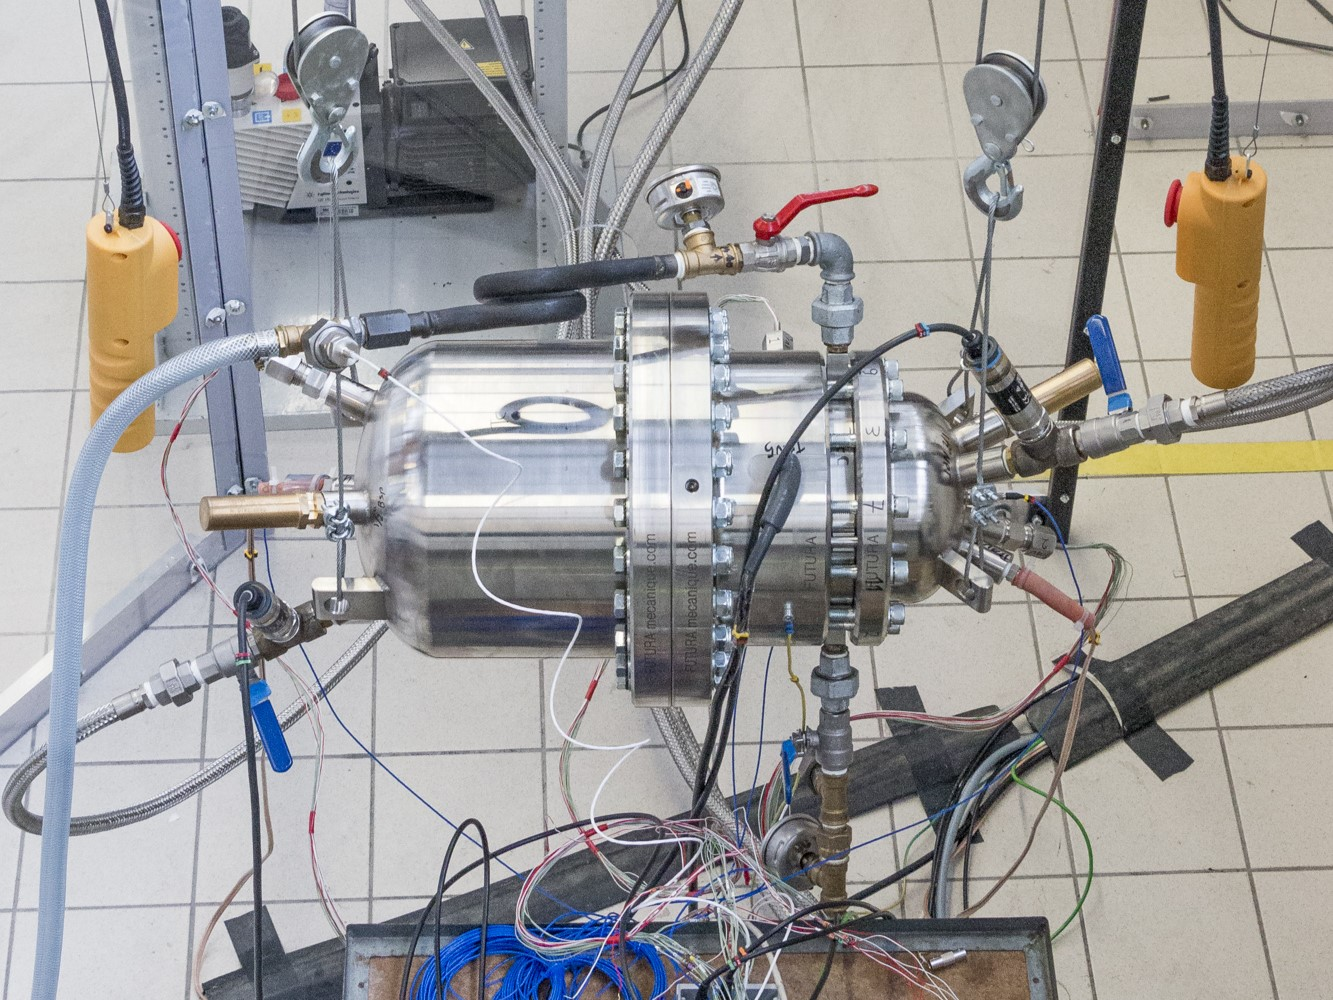
\includegraphics[width=\textwidth]{../fig/fig_SystemeAccroche/Machine_horizBetter_cropped.jpg}
		\caption{}
		\label{fig:TACOTSuspendu_Frigo}
	\end{subfigure}		%
	\begin{subfigure}{.47\textwidth}
		\centering
		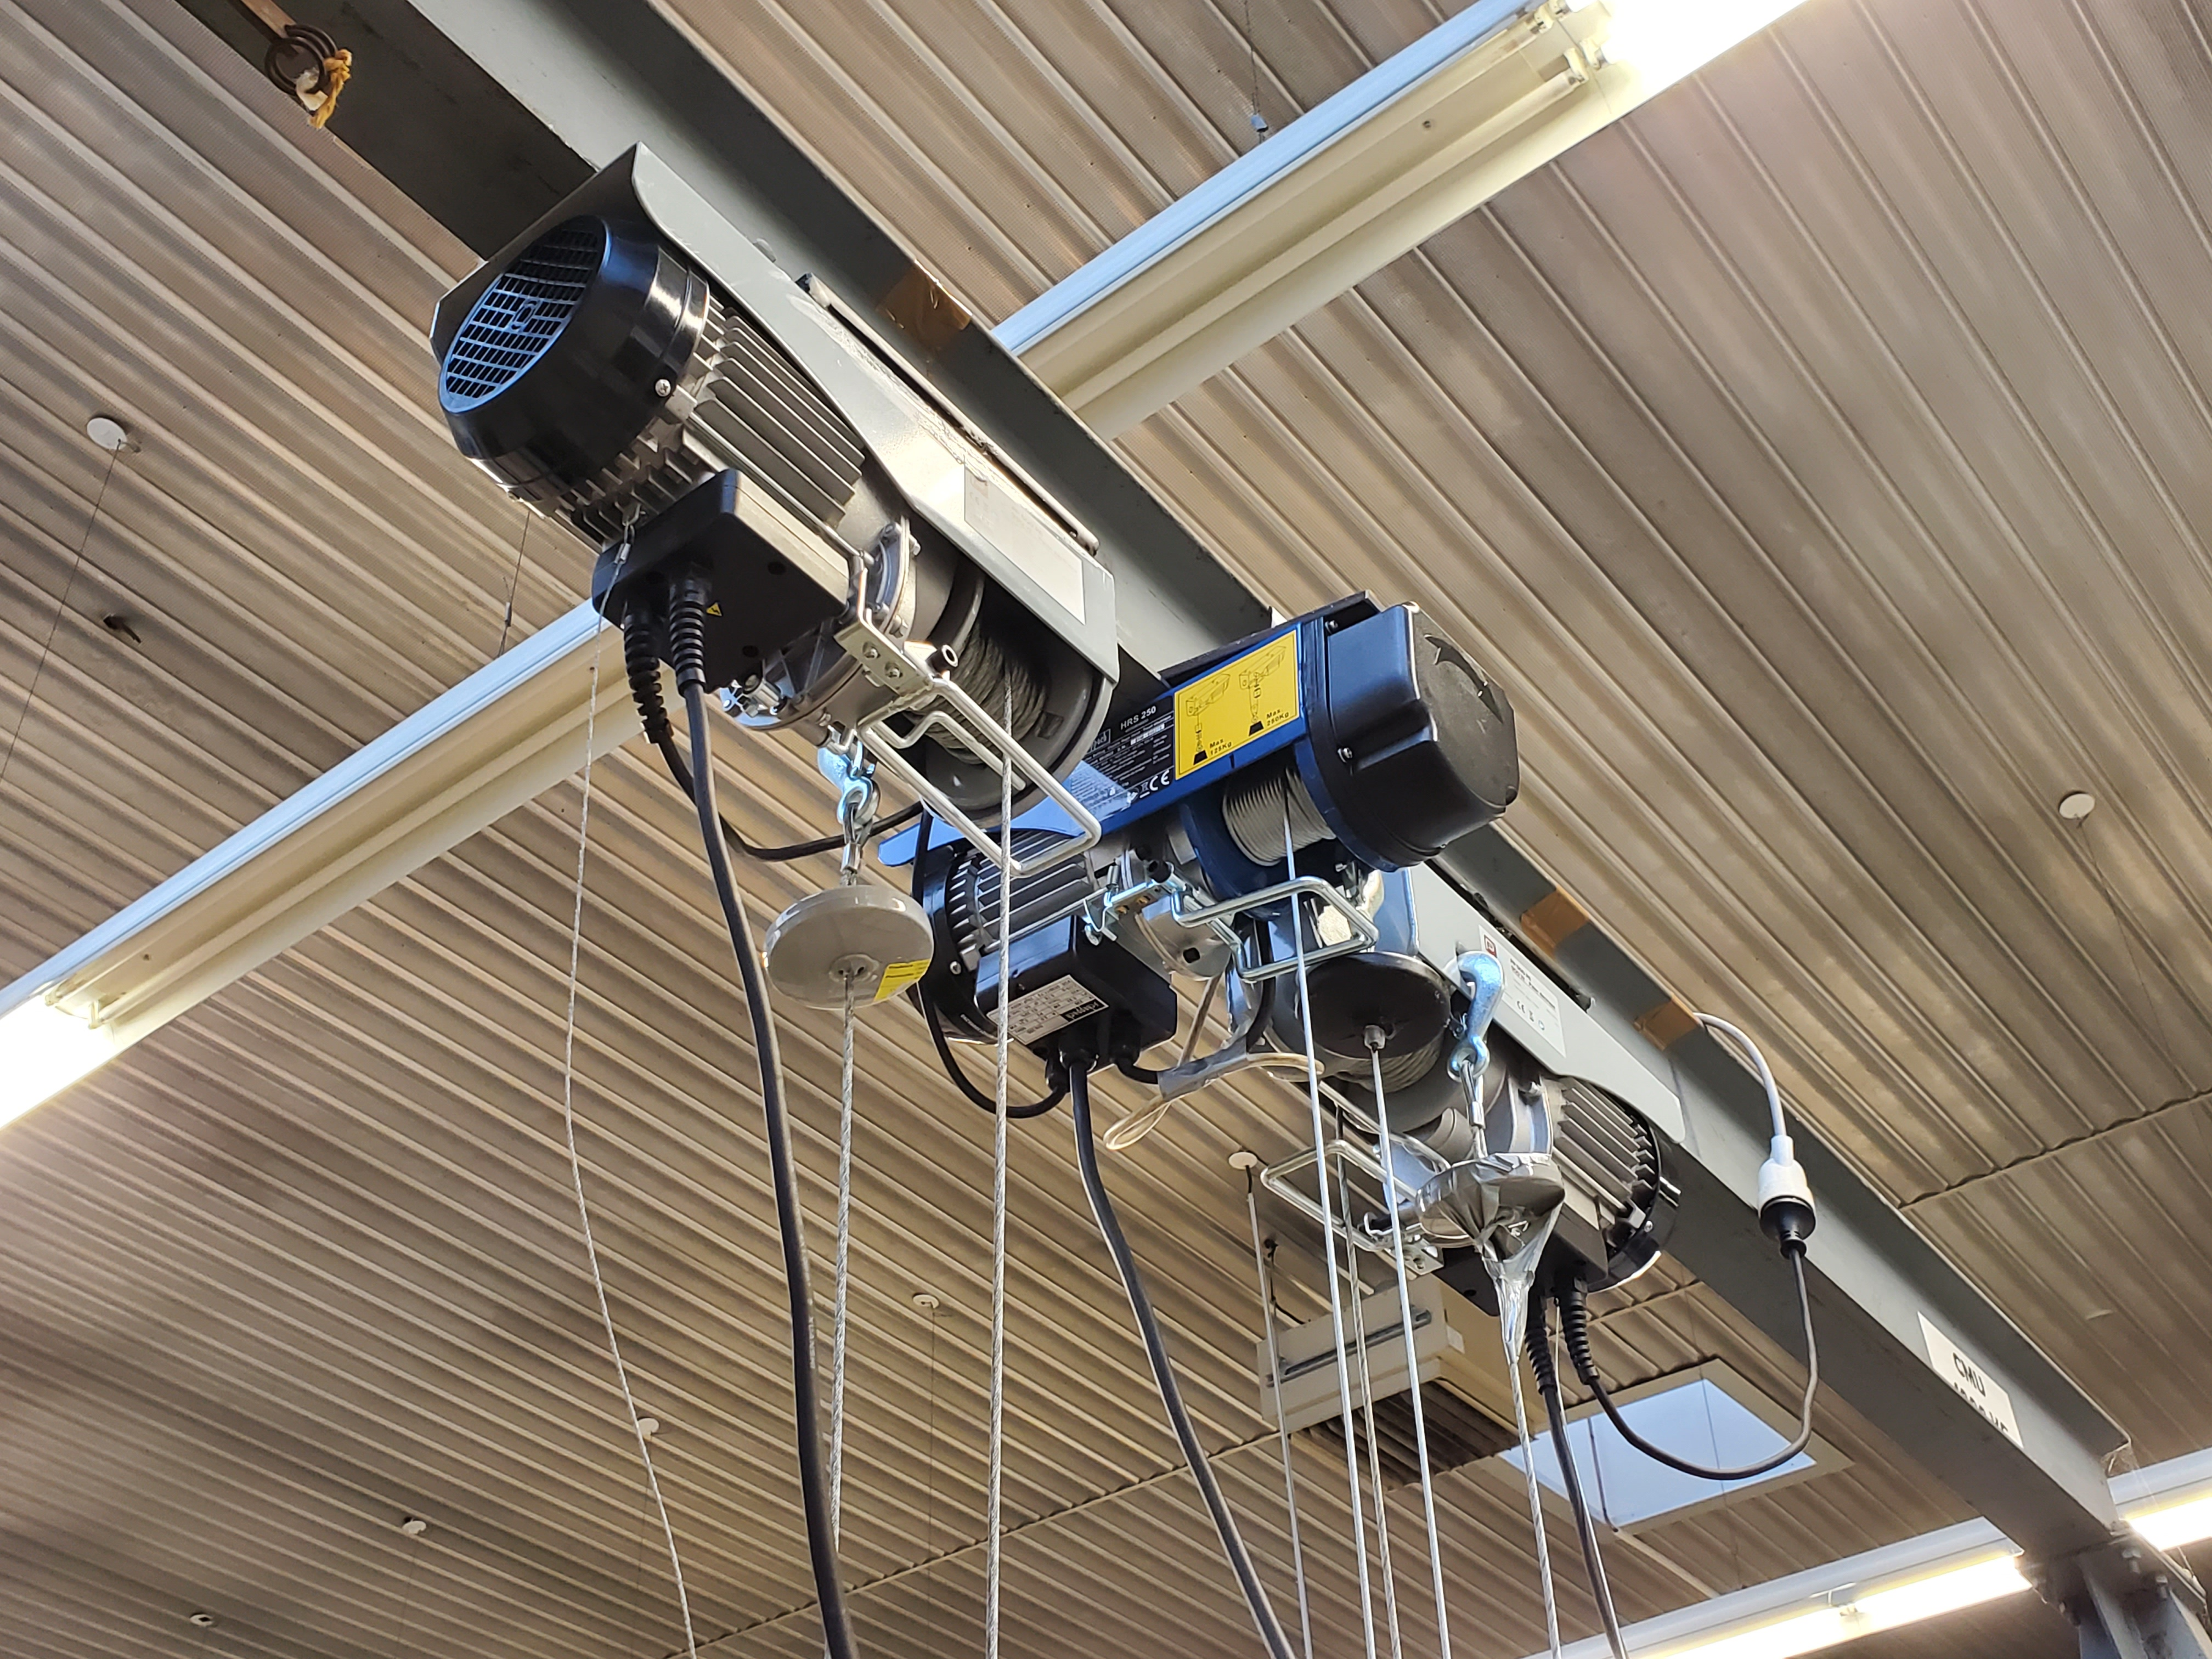
\includegraphics[width=\textwidth]{../fig/fig_SystemeAccroche/Palans.jpg}
		\caption{}
		\label{fig:TACOTSuspendu_Palans}
	\end{subfigure}	    
    \caption{Photographies \subref{fig:TACOTSuspendu_Frigo} du refrigérateur accroché et \subref{fig:TACOTSuspendu_Palans} des palans formant le système de suspension.}
    \label{fig:TACOTSuspendu}
\end{figure}

\subsection{Définition des orientations}

Les orientations choisies au moyen des palans sont décrites par deux angles $\psi_v$ et $\psi_h$. Le premier désigne l'angle entre l'axe horizontal et l'axe de symétrie du réfrigérateur, tandis que le second, la rotation autour de cet axe de symétrie. Les orientations utilisées dans les différentes parties de ce manuscript sont présentées sur la figure~\ref{fig:OrientationCore}. Cette figure, dans laquelle la gravité est toujours dirigée vers le bas de la page, présente également les emplacements et les numéros d'identification des thermocouples utilisés.\medskip

\begin{figure}[!ht]
    \centering
	\begin{subfigure}[c]{.47\textwidth}
		\centering
		\external{fig_OrientationCore_H1}
%    	\externalremake
		\begin{tikzpicture}[scale=2/3]

%    \def\lenreg{2};
%    \def\diam{3};
    \def\spy{2};
    \def\xdist{8cm};
    \def\ydist{-7cm};
%    \def\persp{20};
%    
%    \def\LX{1};
%    \def\LY{2};
%    \def\CoreX{1.5};
%    \def\CoreY{.9*\LY};
%    

	\def\L{2.1};
	\def\R{5};
	\def\HX{.25};
	\def\decalage{\R/2-\L/2};
	
		\draw(6.5,\R/2) node{\includegraphics[width=.8\textwidth]{../fig/fig_OrientationCore/tex/TACOT.png}};
			
		\fill[right color=blue!25,left color=red!25, draw=black] (\decalage,0) rectangle ++(\L,\R);
		\draw[fill=red!25] (\decalage,0) rectangle ++(-\HX,\R);
		\draw[fill=blue!25] (\decalage+\L,0) rectangle ++(\HX,\R);

		\foreach \z [evaluate=\z] in {0,...,4}{
			\foreach \r [evaluate=\r as \num using int(\r+1 + 3*\z)] in {0,...,2}{
				\draw ({\decalage+.5+\L-\z*(1+\L)/4},{-(\R-.4)/2*\r+\R-.2}) node[minimum size=10pt,draw,circle,fill=white,opacity=.7,text opacity=1]{} node(n\z\r){\scriptsize \num};
}}

%		\draw (n01.east) node [right]{0 $\rightarrow$ \begin{tabular}{l}Source\\acoustique\\principale\end{tabular}};
		\draw ($(n01)+(1.5,0)$) node[minimum size=10pt,draw,circle,fill=white,opacity=.7,text opacity=1]{} node(RIX) {\scriptsize 0};% node[anchor=west]{\begin{tabular}{rl}
%		& Source\\
%		$\rightarrow$ & acoustique\\
%		& principale
%		\end{tabular}};
		\draw (n30.north west) node [above, fill=white, fill opacity=.7, text opacity=1]{Ambiant};
		\draw (n10.north east) node [above, fill=white, fill opacity=.7, text opacity=1]{Froid};
\end{tikzpicture}
		\caption{`\texttt{H1}'}
		\label{fig:OrientationCore_H1}
	\end{subfigure}		%
	\begin{subfigure}[c]{.47\textwidth}
		\centering
		\external{fig_OrientationCore_H2}
%    	\externalremake
		\begin{tikzpicture}[scale=2/3]

%    \def\lenreg{2};
%    \def\diam{3};
    \def\spy{2};
    \def\xdist{8cm};
    \def\ydist{-7cm};
%    \def\persp{20};
%    
%    \def\LX{1};
%    \def\LY{2};
%    \def\CoreX{1.5};
%    \def\CoreY{.9*\LY};
%    

	\def\L{1};
	\def\R{5};
	\def\HX{.25};
	\def\decalage{\R/2-\L/2};
	
%	\draw[opacity=0] (\decalage,0) rectangle ++(-\HX,\R); %%% Pour l'alignement vertical
%\draw{[white](\L/2,0) -- ++(0,\R);
	
	\begin{scope}[yslant=-1]
		\begin{scope}[xslant=.71]%, rotate=90, xscale=1]
		\node at (\decalage-\HX,0) (NewO) {};
%		\draw[->, very thick] (NewO.center) -- ++(0,1.2*\R);
%		\draw[->, very thick] (NewO.center) -- ++(1.2*\R,0);
		
		\fill[shading=axis,right color=MatlabBlue,left color=MatlabOrange, shading angle=22.5, draw=black] (\decalage,0) rectangle ++(\L,\R*1.4);
		\draw[fill=MatlabOrange] (\decalage,0) rectangle ++(-\HX,\R*1.4);
		\draw[fill=MatlabBlue] (\decalage+\L,0) rectangle ++(\HX,\R*1.4);

		\foreach \z [evaluate=\z] in {0,...,4}{
			\foreach \r [evaluate=\r as \num using int(\r+1 + 3*\z)] in {0,...,2}{
				\draw ({\decalage+.5+\L-\z*(1+\L)/4},{-(\R*1.4-.4)/2*\r+\R*1.4-.2}) node[minimum size=10pt,draw,circle,fill=white,opacity=.7,text opacity=1]{} node(n\z\r){\scriptsize \num};
}}

%		\draw (n01.east) node [right]{$\rightarrow$ \begin{tabular}{l}Source\\acoustique\\principale\end{tabular}};
		\draw ($(n01)+(.75,0)$) node[minimum size=10pt,draw,circle,fill=white,opacity=.7,text opacity=1]{} node {\scriptsize 0};% node[anchor=west]{\begin{tabular}{rl}
%		& Src\\
%		$\rightarrow$ & ac\\
%		& princ
%		\end{tabular}};
%		\draw (n30.north west) node [above right, fill=white, fill opacity=0, text opacity=1]{\textcolor{MatlabOrange}{\textbf{Ambiant}}};
%		\draw (n10.north east) node [above right, fill=white, fill opacity=0, text opacity=1]{\textcolor{MatlabBlue}{\textbf{Froid}}};
		
	\end{scope}
	\end{scope}
	\begin{pgfonlayer}{background}
		\draw[->, very thick] (NewO.center) -- ++(22.5:1.2*\R) node [above] {$\mathbf e_{y,0}$};
		\draw[->, very thick] (NewO.center) -- ++(90:1.2*\R) node [left] {$\mathbf e_{z,0}$};
		\draw[->, very thick] (NewO.center) -- ++(-45:1.2*\R) node [right] {$\mathbf e_{x,0}$};
  	\end{pgfonlayer}
\end{tikzpicture}
		\caption{`\texttt{H2}'}
		\label{fig:OrientationCore_H2}
	\end{subfigure} \\ \vspace{1cm}
	\begin{subfigure}[c]{.47\textwidth}
		\centering
		\external{fig_OrientationCore_V1}
%    	\externalremake
		%\fill[top color=red!25, bottom color=blue!25, draw=black] (0,0) rectangle ++(\R,\L);
%\draw[fill=blue!25] (0,0) rectangle ++(\R,-\HX);
%\draw[fill=red!25] (0,\L) rectangle ++(\R,\HX);
%
%\foreach \z [evaluate=\z] in {0,...,4}{
%	\foreach \r [evaluate=\r as \num using int(\r+1 + 3*\z)] in {0,...,2}{
%		\draw ({-(\R-.4)/2*\r+\R-.2},{\z*(1+\L)/4-.5}) node(n\z\r){\num};
%}}
%
%\draw (n40.south east) node [right]{AHX};
%\draw (n00.north east) node[right]{CHX};
%\draw (n01.south) node [below]{\shortstack{ $\downarrow$ \\Source acoustique principale}};
%
%\draw (0,\L+2*\HX+\spy) node [anchor=west]{\textbf{(c)} \texttt{V1}};

\begin{tikzpicture}[scale=2/3]

%    \def\lenreg{2};
%    \def\diam{3};
    \def\spy{2};
    \def\xdist{8cm};
    \def\ydist{-7cm};
%    \def\persp{20};
%    
%    \def\LX{1};
%    \def\LY{2};
%    \def\CoreX{1.5};
%    \def\CoreY{.9*\LY};
%    

	\def\L{2};
	\def\R{5};
	\def\HX{.35};
	\def\decalage{\R/2-\L/2};
	
	\begin{scope}[yslant=tan(22.5)]	
		
		\node at (0,-\HX) (NewO) {};
	
		\fill[shading=axis,right color=MatlabBlue,left color=MatlabOrange, shading angle=22.5, draw=black] (0,0) rectangle ++(\R,\L);
		\draw[fill=MatlabBlue] (0,0) rectangle ++(\R,-\HX);
		\draw[fill=MatlabOrange] (0,\L) rectangle ++(\R,\HX);

		\foreach \z [evaluate=\z] in {0,...,4}{
			\foreach \r [evaluate=\r as \num using int(\r+1 + 3*\z)] in {0,...,2}{
				\draw ({-(\R-.4)/2*\r+\R-.2},{\z*(1+\L)/4-.5}) node[minimum size=10pt,draw,circle,fill=white,opacity=.7,text opacity=1]{} node(n\z\r){\scriptsize \num};
}}

%		\draw (n40.south east) node [right, fill=white, fill opacity=0, text opacity=1]{\textcolor{MatlabOrange}{\textbf{Ambiant}}};
%		\draw (n00.north east) node[right, fill=white, fill opacity=0, text opacity=1]{\textcolor{MatlabBlue}{\textbf{Froid}}};
		\draw ($(n01.south)+(0,-1.1)$) node[minimum size=10pt,draw,circle,fill=white,opacity=.7,text opacity=1]{} node (RIX){\scriptsize 0};% node[anchor=north]{\begin{tabular}{c}
%		$\downarrow$\\
%		Source acoustique principale
%		\end{tabular}};

	\end{scope}
	\begin{pgfonlayer}{background}
		\draw[->, very thick] (NewO.center) -- ++(22.5:1.2*\R) node [above] {$\mathbf e_{y,0}$};
		\draw[->, very thick] (NewO.center) -- ++(90:1.2*\R) node [left] {$\mathbf e_{z,0}$};
		\draw[->, very thick] (NewO.center) -- ++(-45:1.2*\R) node [right] {$\mathbf e_{x,0}$};
  	\end{pgfonlayer}		
\end{tikzpicture}
		\caption{`\texttt{V1}'}
		\label{fig:OrientationCore_V1}
	\end{subfigure} %
	\begin{subfigure}[c]{.47\textwidth}
		\centering
		\external{fig_OrientationCore_V2}
%    	\externalremake
		%\fill[top color=blue!25, bottom color=red!25, draw=black] (0,0) rectangle ++(\R,\L);
%\draw[fill=red!25] (0,0) rectangle ++(\R,-\HX);
%\draw[fill=blue!25] (0,\L) rectangle ++(\R,\HX);
%
%\foreach \z [evaluate=\z] in {0,...,4}{
%	\foreach \r [evaluate=\r as \num using int(\r+1 + 3*\z)] in {0,...,2}{
%		\draw ({(\R-.4)/2*\r+.2},{-\z*(1+\L)/4+\L+.5}) node(n\z\r){\num};
%}}
%
%\draw (n01.north) node [above]{\shortstack{Source acoustique principale\\ $\uparrow$}};
%\draw (n42.north east) node [right]{AHX};
%\draw (n02.south east) node [right]{CHX};
%
%\draw (0,\L+2*\HX+\spy) node [anchor=west]{\textbf{(d)} \texttt{V2}};

\begin{tikzpicture}[scale=2/3]

%    \def\lenreg{2};
%    \def\diam{3};
    \def\spy{2};
    \def\xdist{8cm};
    \def\ydist{-7cm};
%    \def\persp{20};
%    
%    \def\LX{1};
%    \def\LY{2};
%    \def\CoreX{1.5};
%    \def\CoreY{.9*\LY};
%    

	\def\L{2.1};
	\def\R{5};
	\def\HX{.25};
	\def\decalage{\R/2-\L/2};

		\fill[top color=MatlabBlue, bottom color=MatlabOrange, draw=black] (0,0) rectangle ++(\R,\L);
		\draw[fill=MatlabOrange] (0,0) rectangle ++(\R,-\HX);
		\draw[fill=MatlabBlue] (0,\L) rectangle ++(\R,\HX);

		\foreach \z [evaluate=\z] in {0,...,4}{
			\foreach \r [evaluate=\r as \num using int(\r+1 + 3*\z)] in {0,...,2}{
				\draw ({(\R-.4)/2*\r+.2},{-\z*(1+\L)/4+\L+.5}) node[minimum size=10pt,draw,circle,fill=white,opacity=.7,text opacity=1]{} node(n\z\r){\scriptsize \num};
}}

		\draw ($(n01.north)+(0,1.1)$) node[minimum size=10pt,draw,circle,fill=white,opacity=.7,text opacity=1]{} node(RIX){\scriptsize 0};% node[anchor=south]{\begin{tabular}{c}
%		Source acoustique principale\\
%		$\uparrow$
%		\end{tabular}};
		\draw (n42.north east) node [right, fill=white, fill opacity=.7, text opacity=1]{\textcolor{MatlabOrange}{\textbf{Ambiant}}};
		\draw (n02.south east) node [right, fill=white, fill opacity=.7, text opacity=1]{\textcolor{MatlabBlue}{\textbf{Froid}}};
%		\draw (n41.south) node [below]{\textcolor{white}{\shortstack{Source acoustique principale\\ $\uparrow$}}};
		
\end{tikzpicture}
		\caption{`\texttt{V2}'}
		\label{fig:OrientationCore_V2}
	\end{subfigure}   
    \caption{Différentes orientations du c\oe{}ur thermoacoustique avec les positions des thermocouples et leurs numéro. Pour chaque cas, la gravité est orientée vers le bas. Les orientations correspondent aux angles \subref{fig:OrientationCore_H1}~$\psi_v=\ang{0}$ et $\psi_h=\ang{0}$ pour l'orientation `\texttt{H1}', \subref{fig:OrientationCore_H2}~$\psi_v=\ang{0}$ et $\psi_h=\ang{+90}$ pour l'orientation `\texttt{H2}', \subref{fig:OrientationCore_V1}~$\psi_v=\ang{-90}$ pour l'orientation `\texttt{V1}', et \subref{fig:OrientationCore_V2}~$\psi_v=\ang{+90}$ pour l'orientation `\texttt{V2}'.}%\textcolor{red}{CHX et AHX OK ou éch. froid et éch. chaud ? + $\psi_i$ dans la caption ou la figure ?}}
    \label{fig:OrientationCore} %
\end{figure}



La première orientation, nommée `\texttt{H1}' et représentée sur la figure~\ref{fig:OrientationCore_H1}, est la même que dans l'article dédié à la conception du réfrigérateur \cite{ramadan_design_2021}. Dans cette configuration, le \textsc{Tacot} est placé à l'horizontale comme sur la figure~\ref{fig:TACOTSuspendu_Frigo}, et les thermocouples sont placés sur un plan vertical coplanaire à la gravité. Cette orientation fait office de référence des orientations, soit $\psi_v=\psi_h=\qty{0}{\degree}$.\smallskip

Ensuite, la deuxième orientation est représentée sur la figure~\ref{fig:OrientationCore_H2}. Dans ce cas, référérencé en tant que `\texttt{H2}', le réfrigérateur est toujours à l'horizontale ($\psi_v=\qty{0}{\degree}$), mais pivoté autour de son axe pour placer les thermocouples sur un plan horizontal auquel la gravité est orthogonale ($\psi_h=\qty{90}{\degree}$).\smallskip

L'orientation `\texttt{V1}' est affichée sur la figure~\ref{fig:OrientationCore_V1}. Cette configuration est radicalement différentes des deux précédentes : l'axe de symétrie du réfrigérateur est vertical, avec l'échangeur froid sous l'échangeur ambiant, soit $\psi_v=\qty{-90}{\degree}$. \smallskip

Enfin, l'orientation `\texttt{V2}' affichée sur la figure~\ref{fig:OrientationCore_V2} est l'orientation inverse de la précédente. L'axe de symétrie du réfrigérateur est encore vertical, mais la source acoustique principale est cette fois au dessus du noyau thermoacoustique et $\psi_v=\qty{+90}{\degree}$.

\subsection{Acquisitions}
Les acquisitions sont réalisées en plusieurs temps. Tout d'abord et pour toutes les expériences,  l'état initial de toutes les grandeurs est acquis sur une minute et sauvegardé sous un label `\texttt{init}' à chaque début de journée de campagne. Cela permet de garder en mémoire toutes les conditions expérimentales initiales dont les valeurs peuvent potentiellement influer sur le comportement du réfrigérateur, comme par exemple la température ambiante ou la pression statique. \medskip

Ensuite, en prévision de la mesure de flux de chaleur $\dot Q_a$ extrait par l'échangeur ambiant (voir l'annexe~\ref{chap:AHX}), l'eau est préalablement mise en circulation dans cet échangeur après avoir démarré une acquisition des 30 capteurs jusqu'à stabilisation de la distribution de température dans le noyau. L'acquisition est ensuite interrompue et enregistrée avec un label `\texttt{Water}'. \bigskip

L'étape suivante dépend du type d'expérience menée : les mesures peuvent être sans ou avec acoustique, et ce, pour  différentes amplitudes de pression oscillante. En revanche, certains des paramètres d'excitation restent constants pour toutes les expériences :  le gaz est également le même dans toutes les expériences. Il est composé de \qty{65}{\percent} d'hélium et de \qty{35}{\percent} d'argon, car dans ces proportions le nombre de Prandtl est minimum \cite{belcher_working_1999} ; ce mélange est ensuite pressurisé à \qty{40}{\bar}. Dans le cas des expériences avec acoustique, le modèle \textsc{DeltaEC} prédit les meilleurs performances à la fréquence $f=\qty{47}{\hertz}$, c'est-à-dire la fréquence de résonance du système. C'est par ailleurs le seul point de fonctionnement où l'impédance électrique est supérieure à la limite basse admise par l'amplificateur, soit \qty{2}{\ohm}. Ensuite, le déphasage inter-source $\varphi_{2-1}$ est également fixé à \ang{-60} pour toutes les expériences, également indiqué comme déphasage optimale par les simulations et que des expériences préliminaires confirment.

\subsubsection{Mesures sans acoustique}\label{chap:MesureSansAcou}
Pour ces mesures de type `\texttt{heat\_{}only}', la charge thermique est appliquée au noyau sans alimenter les sources acoustiques. Cette charge thermique consiste en l'alimentation électrique de cartouches chauffantes contenues dans l'échangeur froid par une puissance connue, tandis qu'un débit d'eau de \qty{7}{\litre\per\minute} s'écoule dans l'échangeur ambiant qui se trouve de l'autre côté du noyau. 

Ces mesures doivent permettre d'étudier la distribution de température en l'absence d'écoulement oscillant, ainsi que de calculer les valeurs de conductivité thermique $k_x$ et $k_r$ ou les coefficients de pertes latérales $h_x$ et $h_r$.\medskip

Dans ce type d'expériences, les noms des zones \og froide \fg{} et \og ambiante \fg{} sont conservés pour des raisons de cohérence avec les schémas présentés auparavant, mais l'eau circulant dans l'échangeur ambiant et les cartouches chauffantes se trouvant dans l'échangeur froid, la direction du gradient de température dans le noyau thermoacoustique est inversée par rapport aux expériences avec acoustique. %Toutefois, les ordres de grandeur des différences de température sont les mêmes que pour les expériences avec acoustique, c'est-à-dire 

%Pour garder un moyen de comparaison avec les mesures avec acoustique, le mélange de gaz est le même.

\subsubsection{Mesures avec acoustique}\label{chap:MesureAvecAcou} 
Une acquisition étiquetée `\texttt{Acou}' est démarrée, puis les sources sont alimentées jusqu'à l'amplitude souhaitée. Au bout d'une heure, l'acquisition est arrêtée et sauvegardée. En l'absence d'expérience avec charge thermique, c'est la fin de l'expérience : toutes les sources acoustiques et circulations d'eau sont progressivement arrêtées et le réfrigérateur est laissé pour un retour à l'état initial.

Au cours de cette étude, trois amplitudes acoustiques sont choisies. La première correspond à un \textit{drive ratio} $DR=\frac{p}{P_0}=\qty{.4}{\percent}$, soit une amplitude très faible où l'effet thermoacoustique est à peine visible -- soit un gradient de température de l'ordre de \qty{5}{\degreeCelsius}. Ainsi, l'hypothèse concernant la linéarité acoustique est mieux vérifiée et peut \textit{a priori} être plus aisément comparé à la théorie linéaire. À l'inverse, le \textit{drive ratio} de la deuxième amplitude est le plus élevé avec $DR=\qty{3.5}{\percent}$, et est celui pour lequel les performances du réfrigérateur ($COP$, $Q_f$, ...) sont les plus élevées obtenues avec cette machine \cite{ramadan_design_2021}, mais aussi qui présentent de forts écarts à la théorie. La troisième est choisie à un \textit{drive ratio} intermédiaire où $DR=\qty{2}{\percent}$. 

Ensuite, une charge thermique peut être appliquée au noyau, par le biais de l'échangeur froid. Il contient six cartouches chauffantes connectées en parallel et alimentées électriquement par un transformateur. Pour une expérience donnée, une puissance thermique est choisie selon la relation

\begin{equation}
	Q_f = \frac{E^2}{R},
	\label{eq:Qf_définitionEsurR}
\end{equation}
où $E$ est la tension appliquée aux cartouches et $R=\qty{22.4}{\ohm}$ la résistance des cartouches en parallel. \echaf{à continuer}



\begin{comment}
\subsubsection{Paramètres d'acquisition}
Comme dit précédemment, la fréquence de fonctionnement du \textsc{Tacot} est de \qty{47}{\hertz}, ce qui implique une fréquence d'échantillonnage au moins deux fois supérieure. Cependant, les cartes d'acquisition sont rassemblées sur une baie d'instrumentation, contraignent la fréquence d'échantillonage utilisée. Celles concernant les mesures de quantité oscillantes (pression acoustique, accélération \echaf{à vérifier}) imposent que la fréquence d'échantillonage $f_s$ soit au moins égale à \qty{1651}{\Hz}\footnote{Les acquisitions des \num{30} capteurs durent \qty{1}{\hour}, et les données sont encodées sur \qty{32}{\bit} flottants. Au total, chaque acquisition pèse \qty{713}{\mega\byte}, taille à laquelle il faut ajouter quelques \unit{\mega\byte} pour le protocole \texttt{tdms} et l'entête contenant les informations de mesure.}.
\end{comment}







